\setcounter{section}{3}
\setlength{\parindent}{0pt}
\setlength{\parskip}{6pt}

\section{FrontEnd}

\subsection{Descrizione FrontEnd}
Il FrontEnd della Progressive Web App (PWA) Rinova è stato concepito per offrire un'esperienza utente reattiva, intuitiva e pienamente accessibile in ottica \textit{Mobile-First}. 

L'interfaccia utente non si limita all'utilizzo di librerie pre-confezionate: i componenti di base forniti da \textbf{Shadcn UI} sono stati profondamente personalizzati ed estesi tramite Tailwind CSS per creare una libreria di componenti custom (card, form, widget energetici, tabelle) coerente con la complessa identità visiva e funzionale del progetto.

\subsection{Navigazione}
La navigazione è separata concettualmente in due macro-aree:
\begin{itemize}
    \item \textbf{Area Pubblica (Auth):} Gestisce l'onboarding, la registrazione, il login e il recupero delle credenziali.
    \item \textbf{Area Riservata:} Costituisce il core dell'applicativo e include la Dashboard energetica, lo Storico, la Gestione Impianti e la vista Comunità Energetica.
\end{itemize}

\subsection{Logiche di Visualizzazione e Funzionalità}
Per garantire una User Experience ottimale nella consultazione dei dati energetici, le viste sono state strutturate secondo le seguenti logiche:
\begin{itemize}
    \item \textbf{Dashboard (Live):} I KPI principali (produzione, consumo, stato batteria) mostrano un valore \textit{cumulativo} aggregato di tutti gli impianti dell'utente. Al contrario, per garantire un monitoraggio granulare, viene renderizzato un grafico live distinto per ogni singolo impianto registrato.
    \item \textbf{Storico Produzione (Analytics):} Presenta un grafico unificato. Di default la vista mostra il cumulativo storico di tutti gli asset dell'utente, con la possibilità di utilizzare filtri specifici per isolare e analizzare le performance di un singolo impianto.
    \item \textbf{Gestione Impianti:} Questa sezione integra funzionalità avanzate. Oltre alla visualizzazione dei dettagli tecnici e della posizione esatta su mappa (tramite \textbf{Leaflet}), l'utente può interagire con lo stato dell'asset, ad esempio segnalando un guasto o un periodo di manutenzione (sospendendo temporaneamente il calcolo dell'impianto) per poi riattivarlo a intervento concluso.
    \item \textbf{Comunità Energetica (CER):} L'attuale implementazione funge da \textit{Minimum Viable Product} (MVP) per l'amministrazione interna dei membri. Consapevoli della reale complessità burocratica e in attesa di future integrazioni con la cartografia e i POD del GSE, si è scelto consapevolmente di non banalizzare il processo di adesione con automatismi fittizi, concentrando lo sforzo sulla visualizzazione del bilancio energetico e della bacheca annunci interna.
\end{itemize}

\subsection{Schermate Principali}
Di seguito sono illustrate le schermate principali. Per evidenziare la natura PWA e pienamente responsiva dell'applicazione, per ogni vista è proposto il confronto diretto tra il layout Desktop e quello Mobile.

\begin{figure}[H]
    \centering
    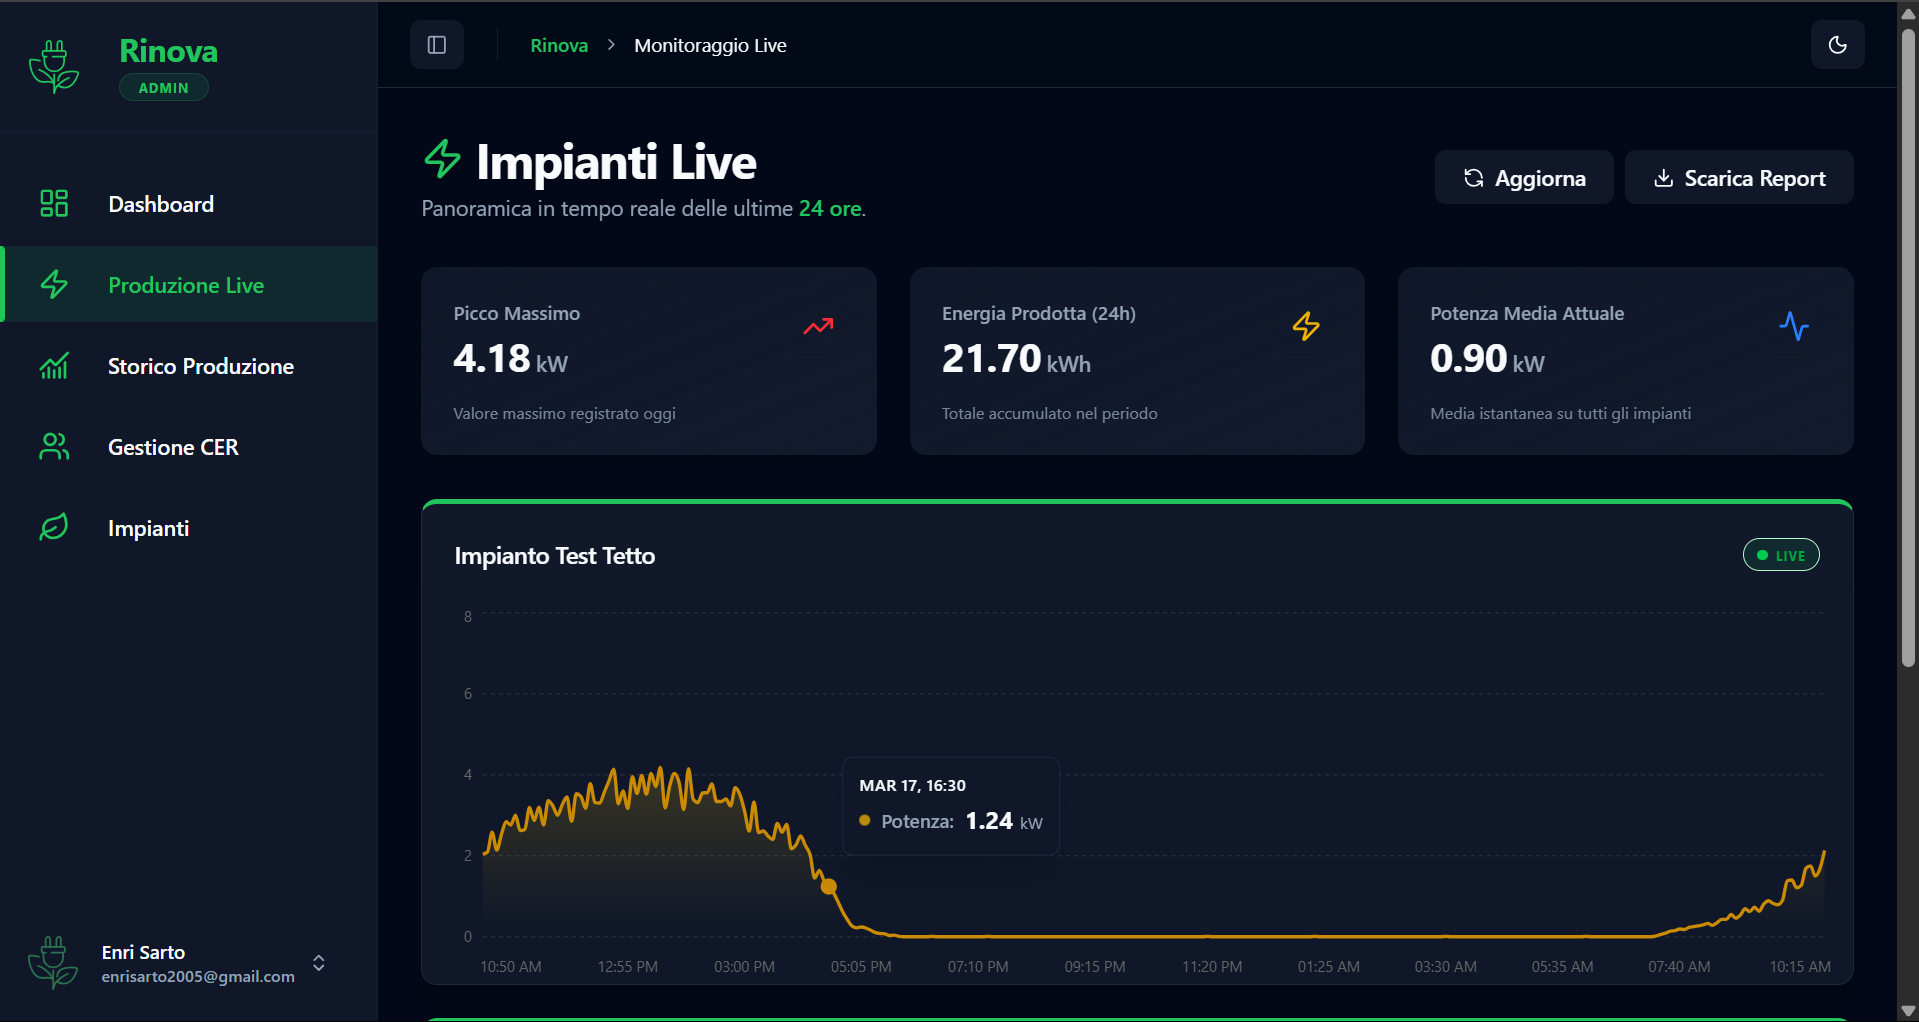
\includegraphics[width=0.95\textwidth]{images/frontend/desktop/live_desktop_dark.png}
    \caption{Dashboard Live: Vista Desktop. Si notano i KPI cumulativi e i grafici di produzione renderizzati per singolo impianto.}
\end{figure}

\begin{figure}
    \centering
    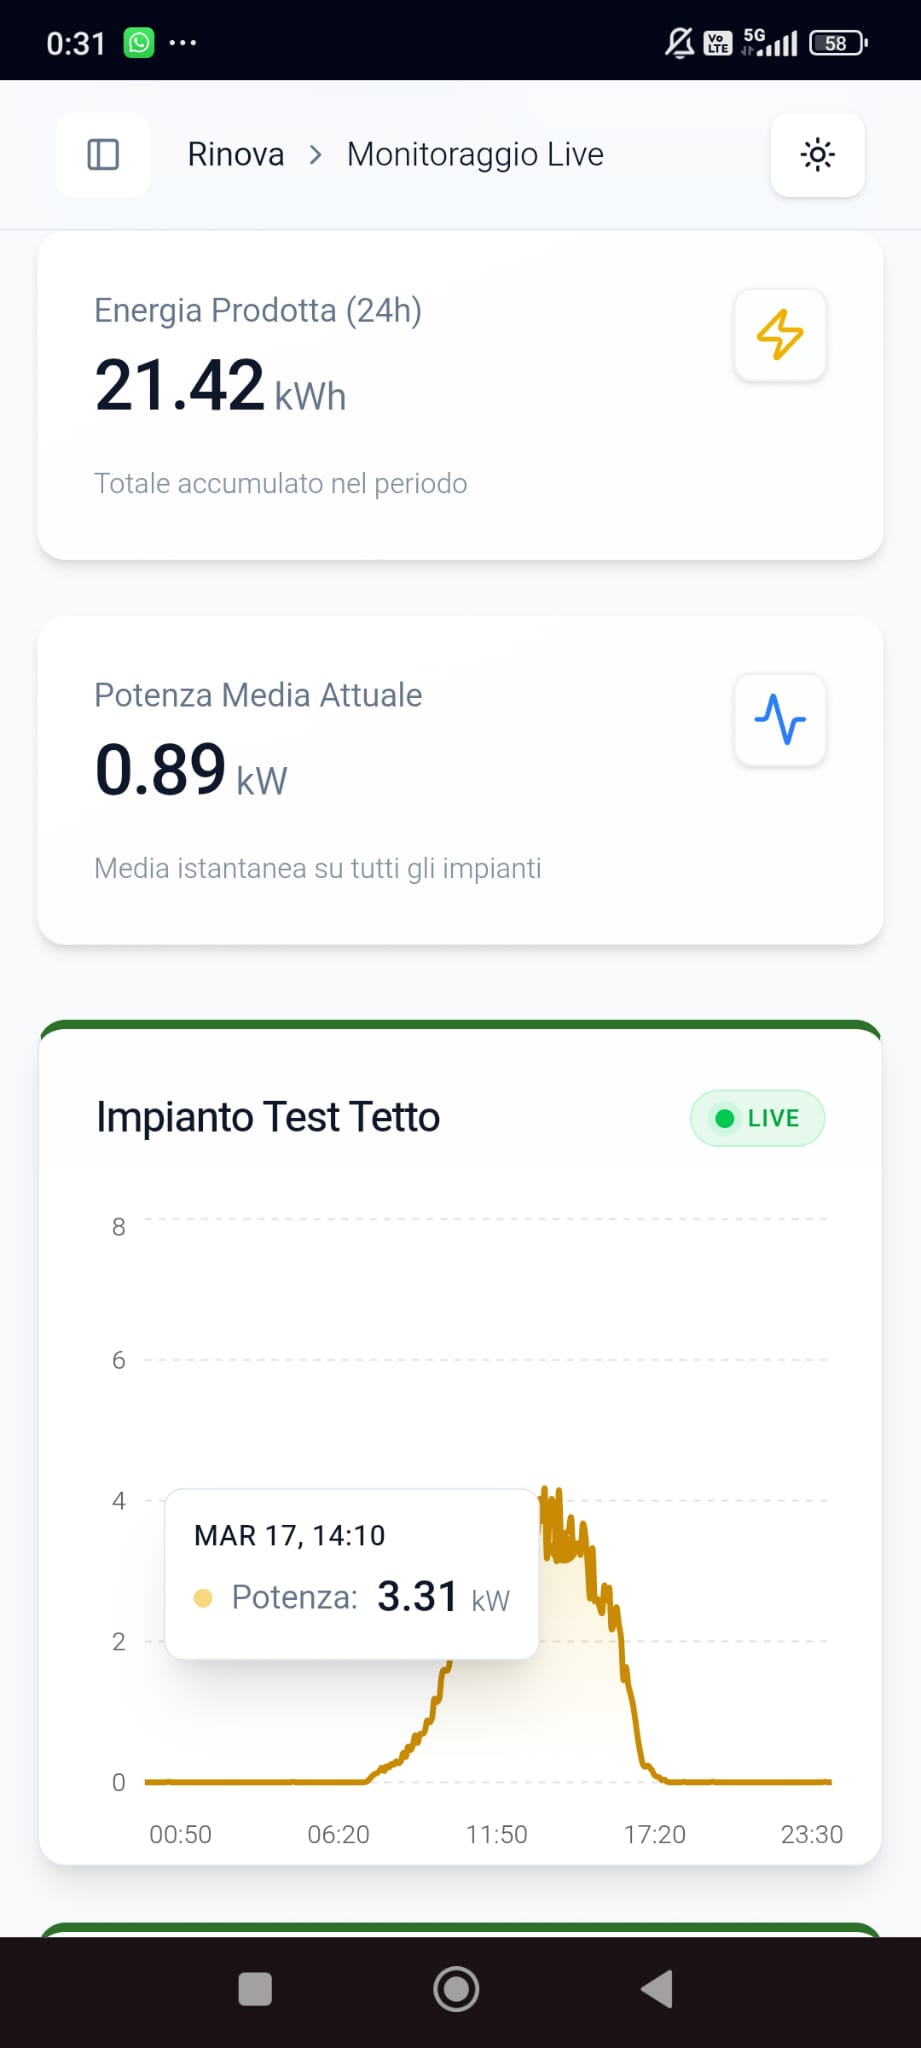
\includegraphics[width=0.45\textwidth]{images/frontend/mobile/live_mobile_grafico_light.jpeg}
    \hspace{0.5cm}
    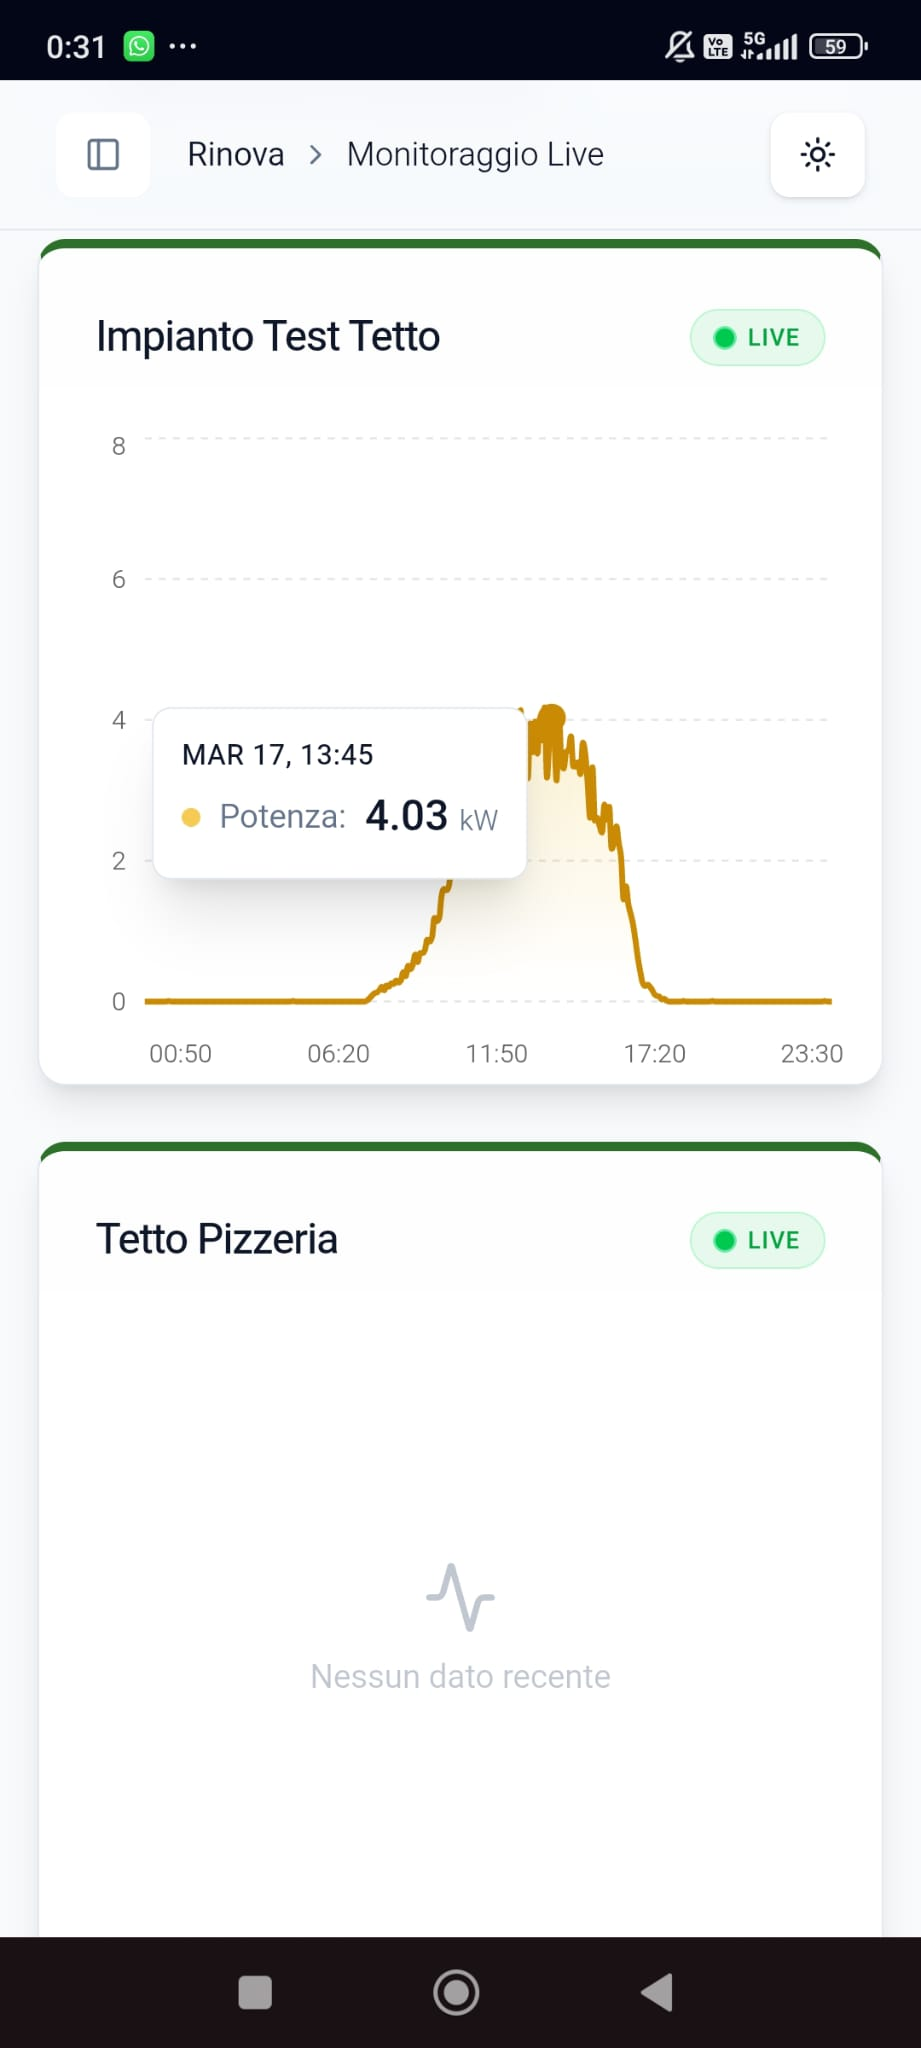
\includegraphics[width=0.45\textwidth]{images/frontend/mobile/live_mobile_grafici_light_2.jpeg}
    \caption{Dashboard Live: Vista Mobile. Si notano i KPI cumulativi e i grafici di produzione renderizzati per singolo impianto.}
\end{figure}

\begin{figure}[H]
    \centering
    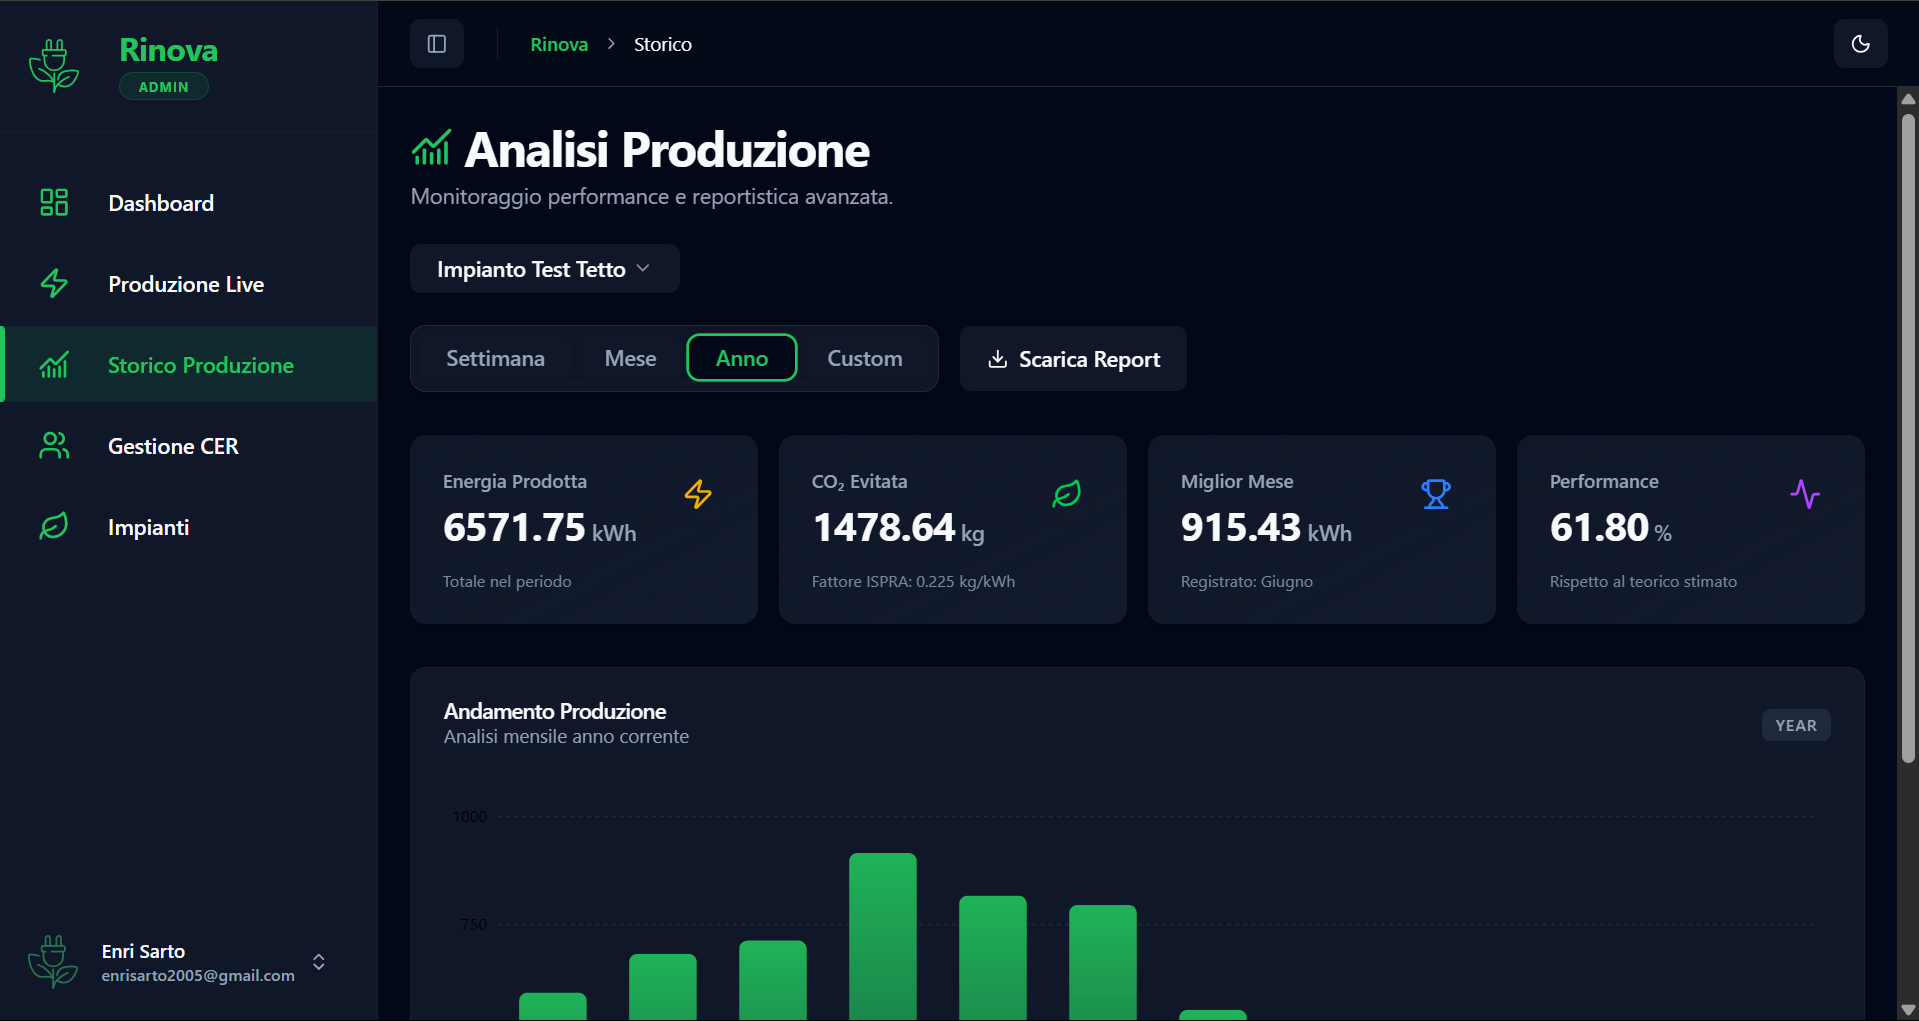
\includegraphics[width=0.95\textwidth]{images/frontend/desktop/storico_desktop_kpi_dark.png}
    
    \vspace{0.5cm}
    
    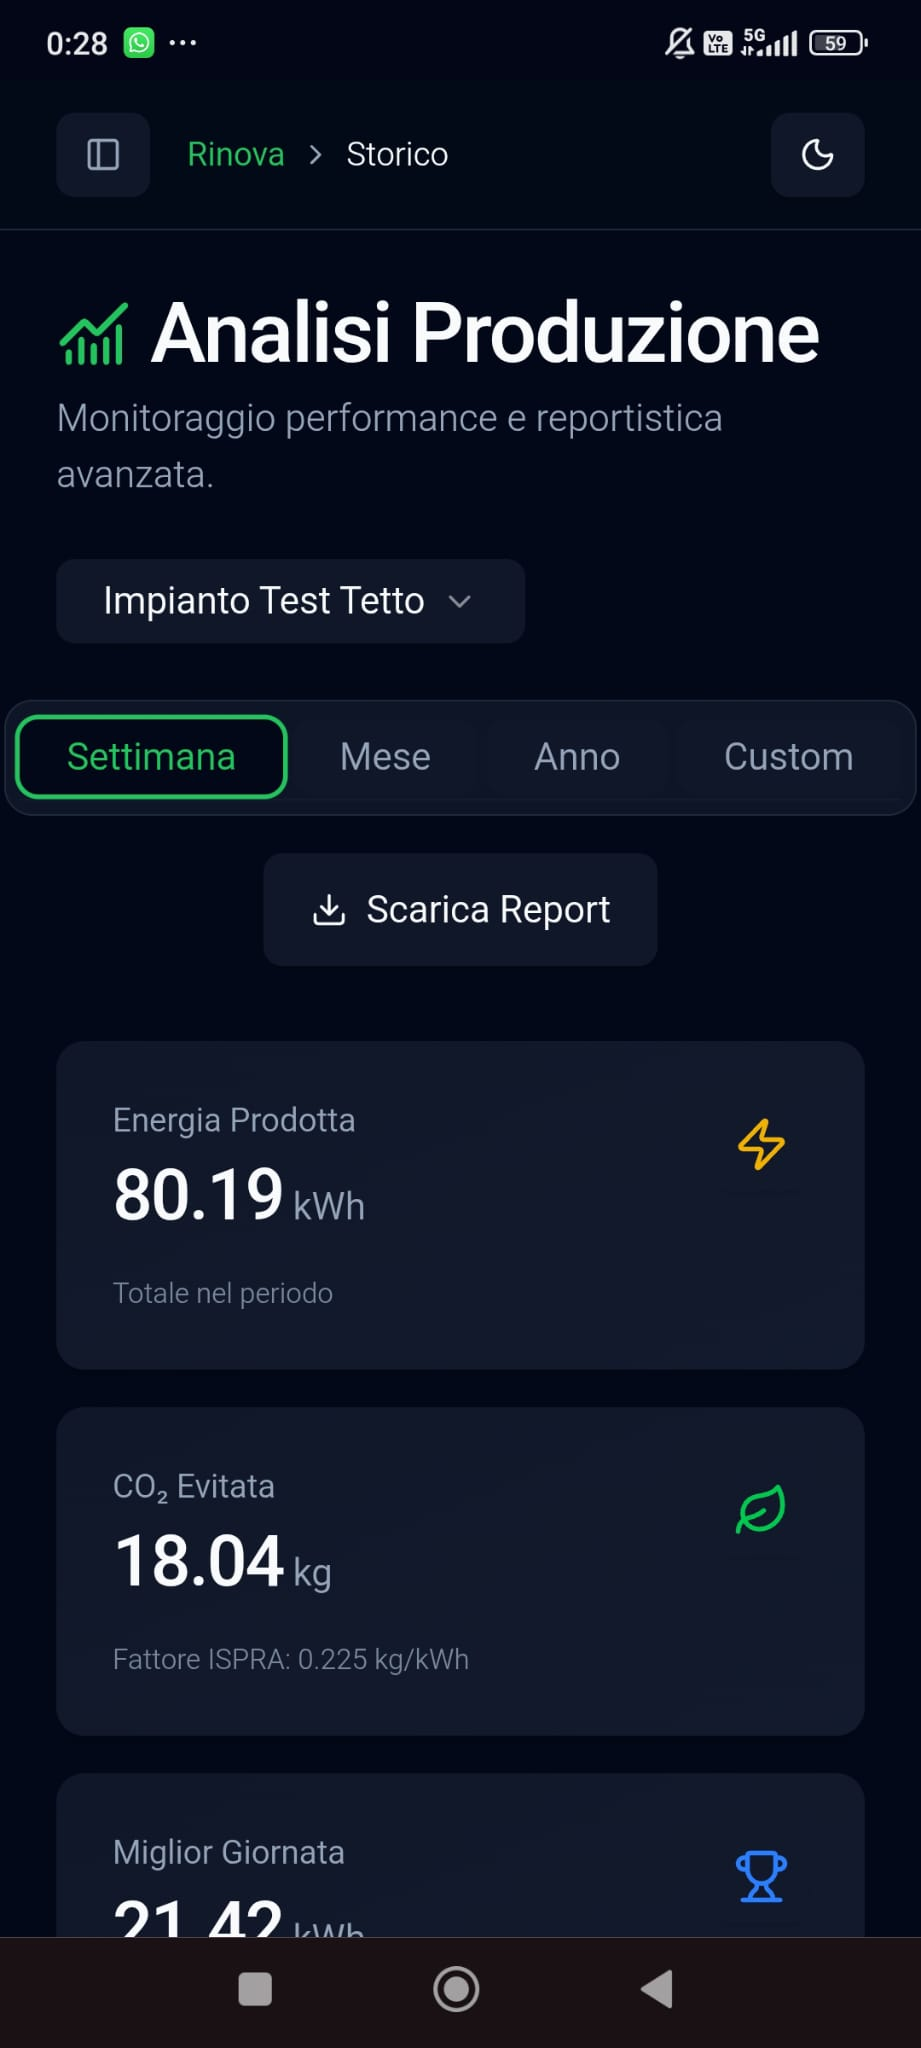
\includegraphics[width=0.35\textwidth]{images/frontend/mobile/storico_mobile_periods_dark.jpeg}
    \hspace{0.5cm}
    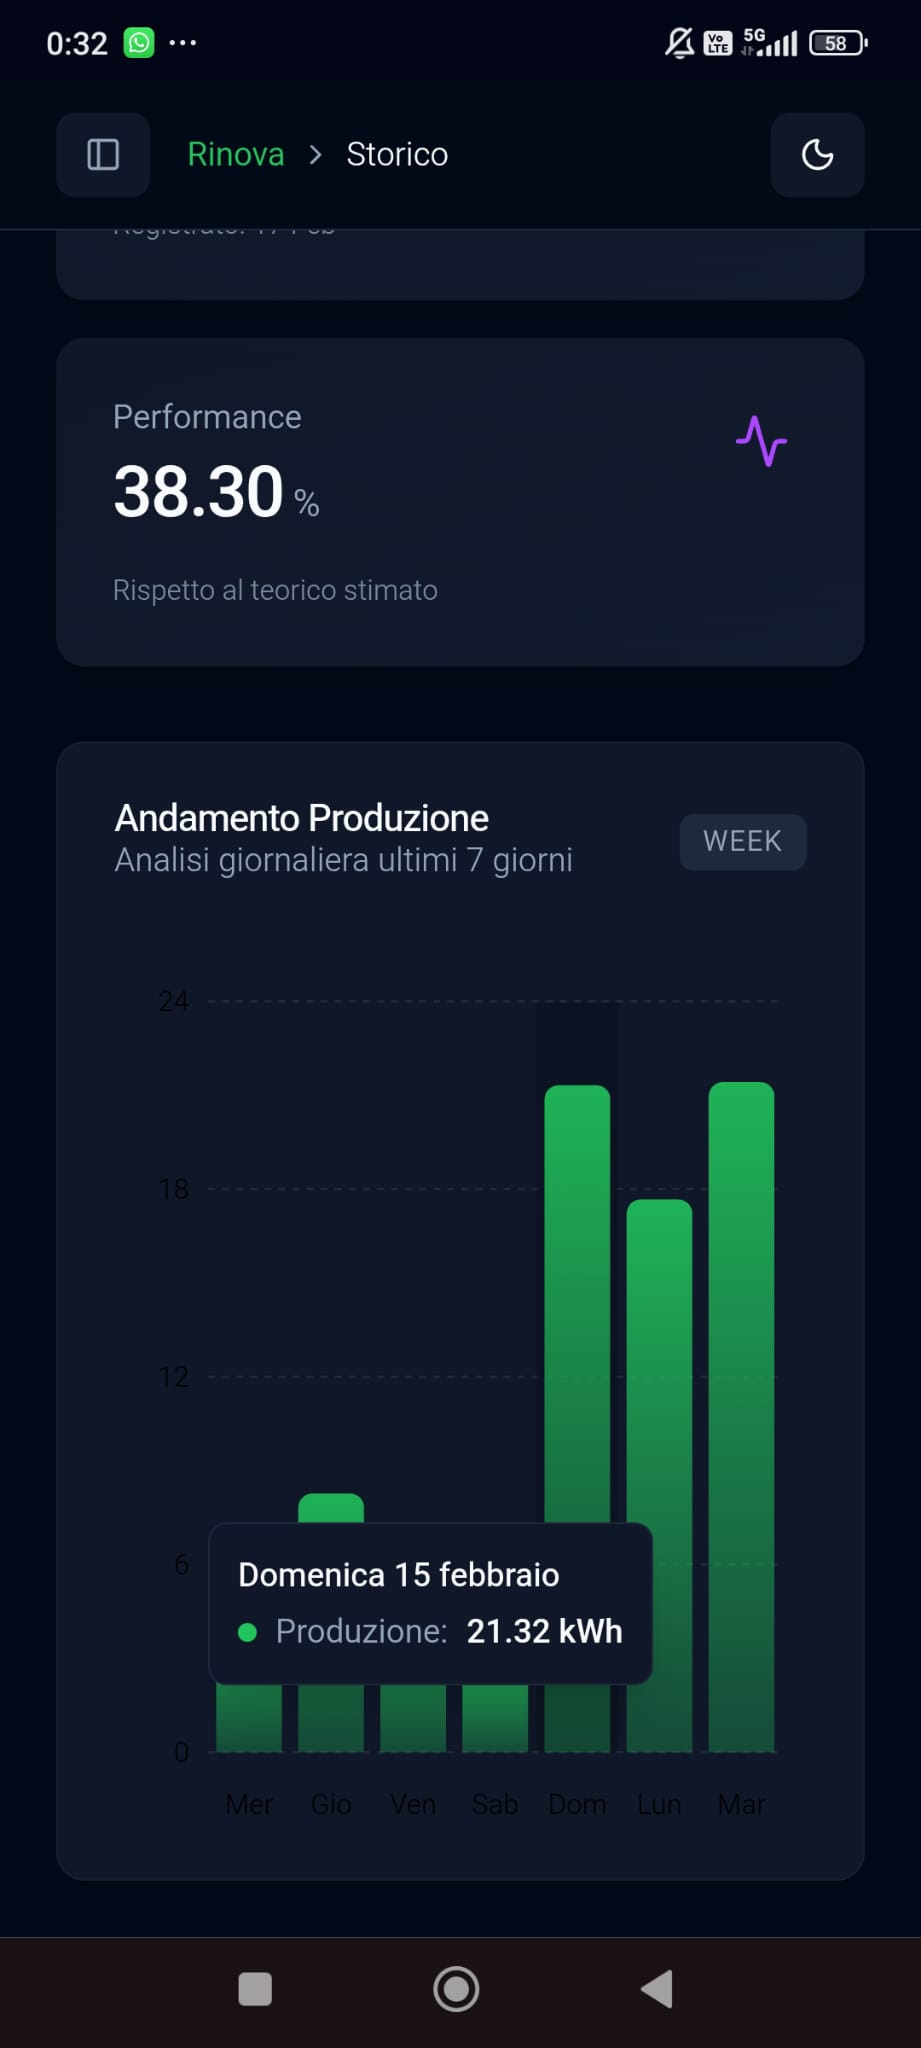
\includegraphics[width=0.35\textwidth]{images/frontend/mobile/storico_mobile_grafico_dark.jpeg}
    
    \caption{Storico Produzione: Vista Desktop (sopra) e Viste Mobile (sotto). Grafico unificato con possibilità di filtraggio per singolo asset.}
\end{figure}

\begin{figure}[H]
    \centering
    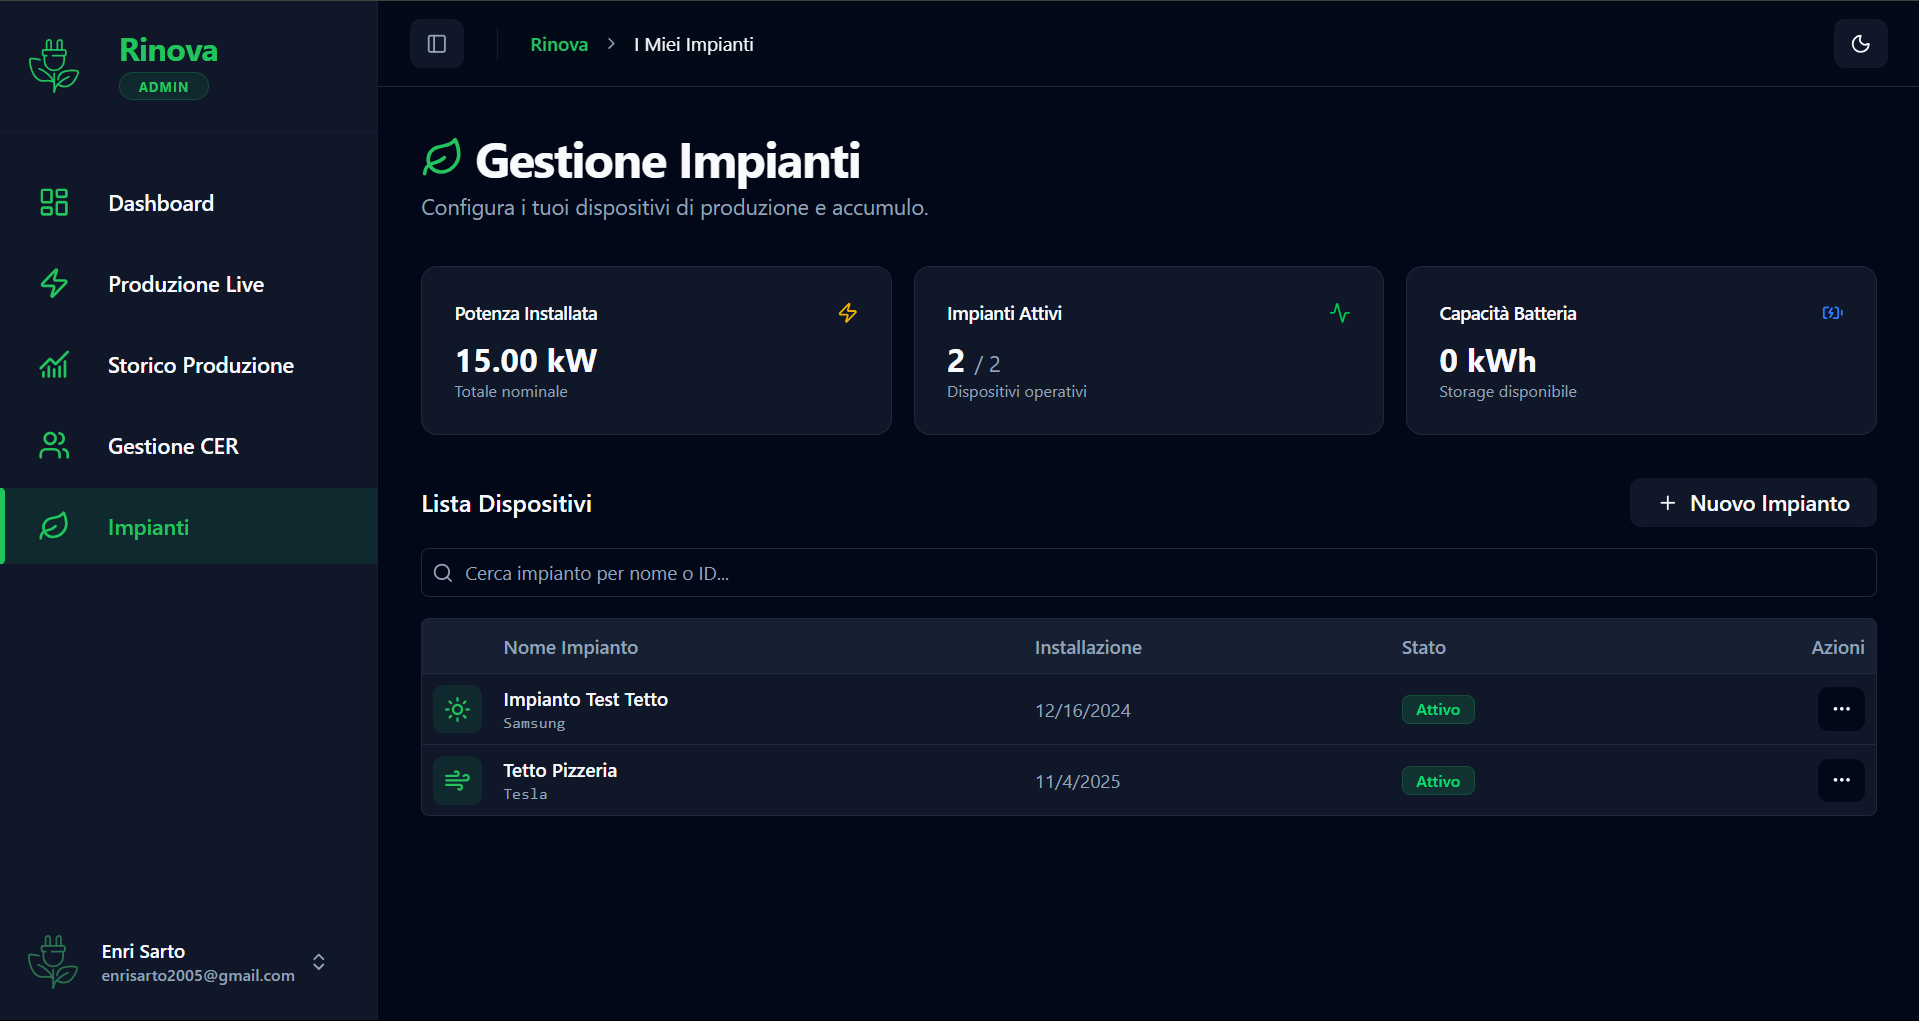
\includegraphics[width=0.95\textwidth]{images/frontend/desktop/impianti_desktop_dark.png}
    
    \vspace{0.5cm}
    
    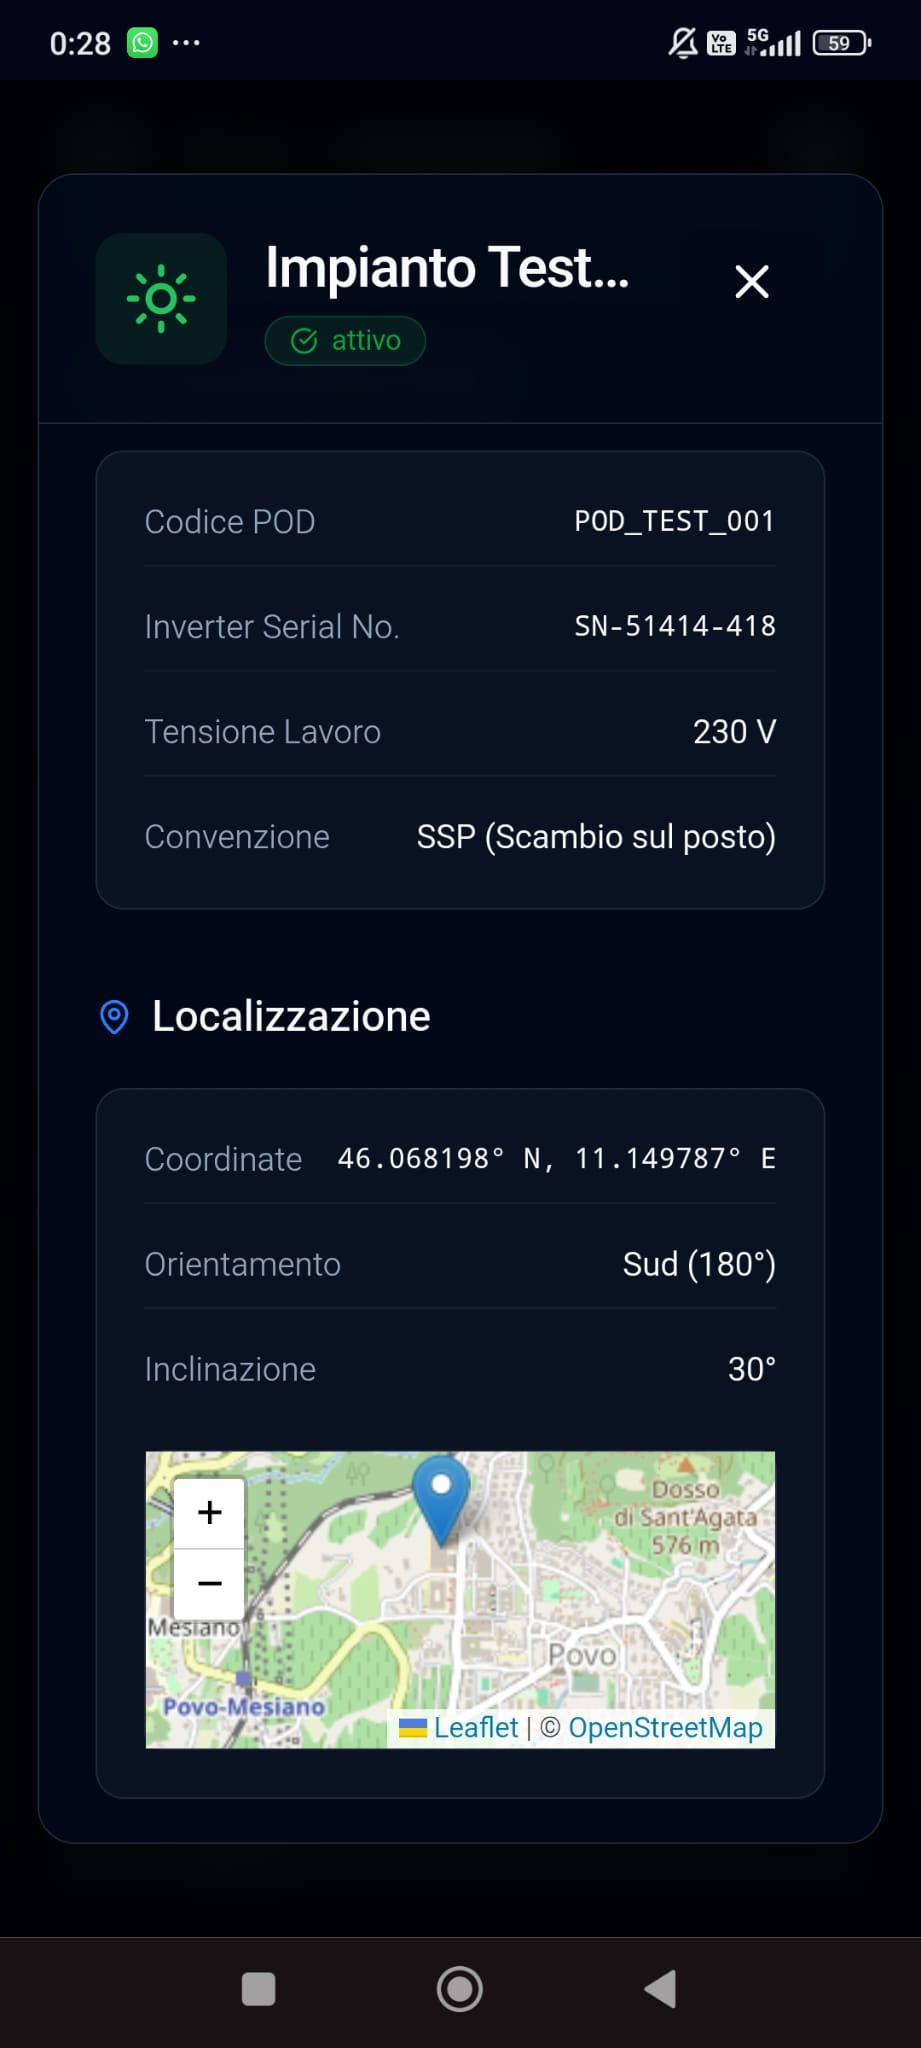
\includegraphics[width=0.35\textwidth]{images/frontend/mobile/impianto_mobile_details_dark.jpeg}
    
    \caption{Gestione Impianti: Vista Desktop (sopra) con una visualizzazione tabellare per il riepilogo della potenza installata, dello stato operativo e Vista Dettaglio Mobile (sotto), con dettagli tecnici dell'impianto e integrazione mappa Leaflet per la posizione. Funzionalità di segnalazione guasti e manutenzioni sono accessibili in layout Desktop e Mobile tramite menù a tendina.}
\end{figure}

\begin{figure}[H]
    \centering
    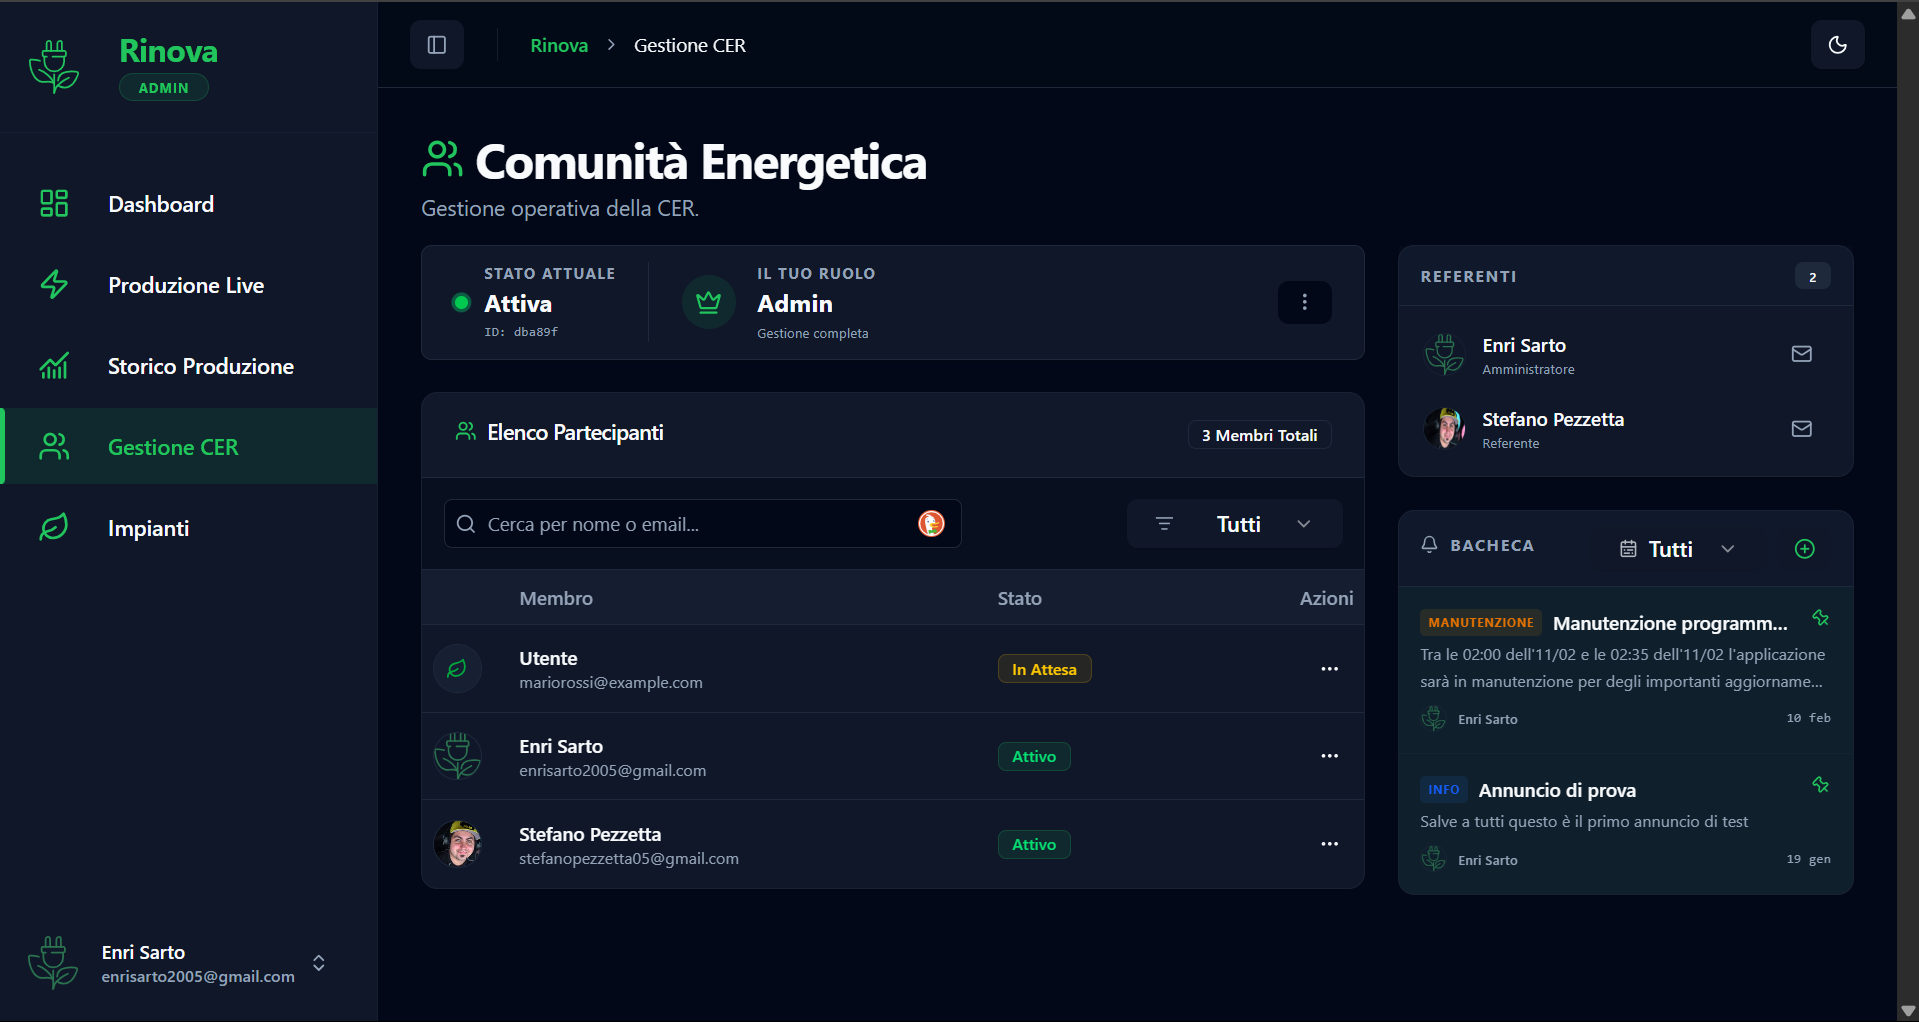
\includegraphics[width=0.95\textwidth]{images/frontend/desktop/cer_desktop_dark.png}
    
    \vspace{0.5cm}
    
    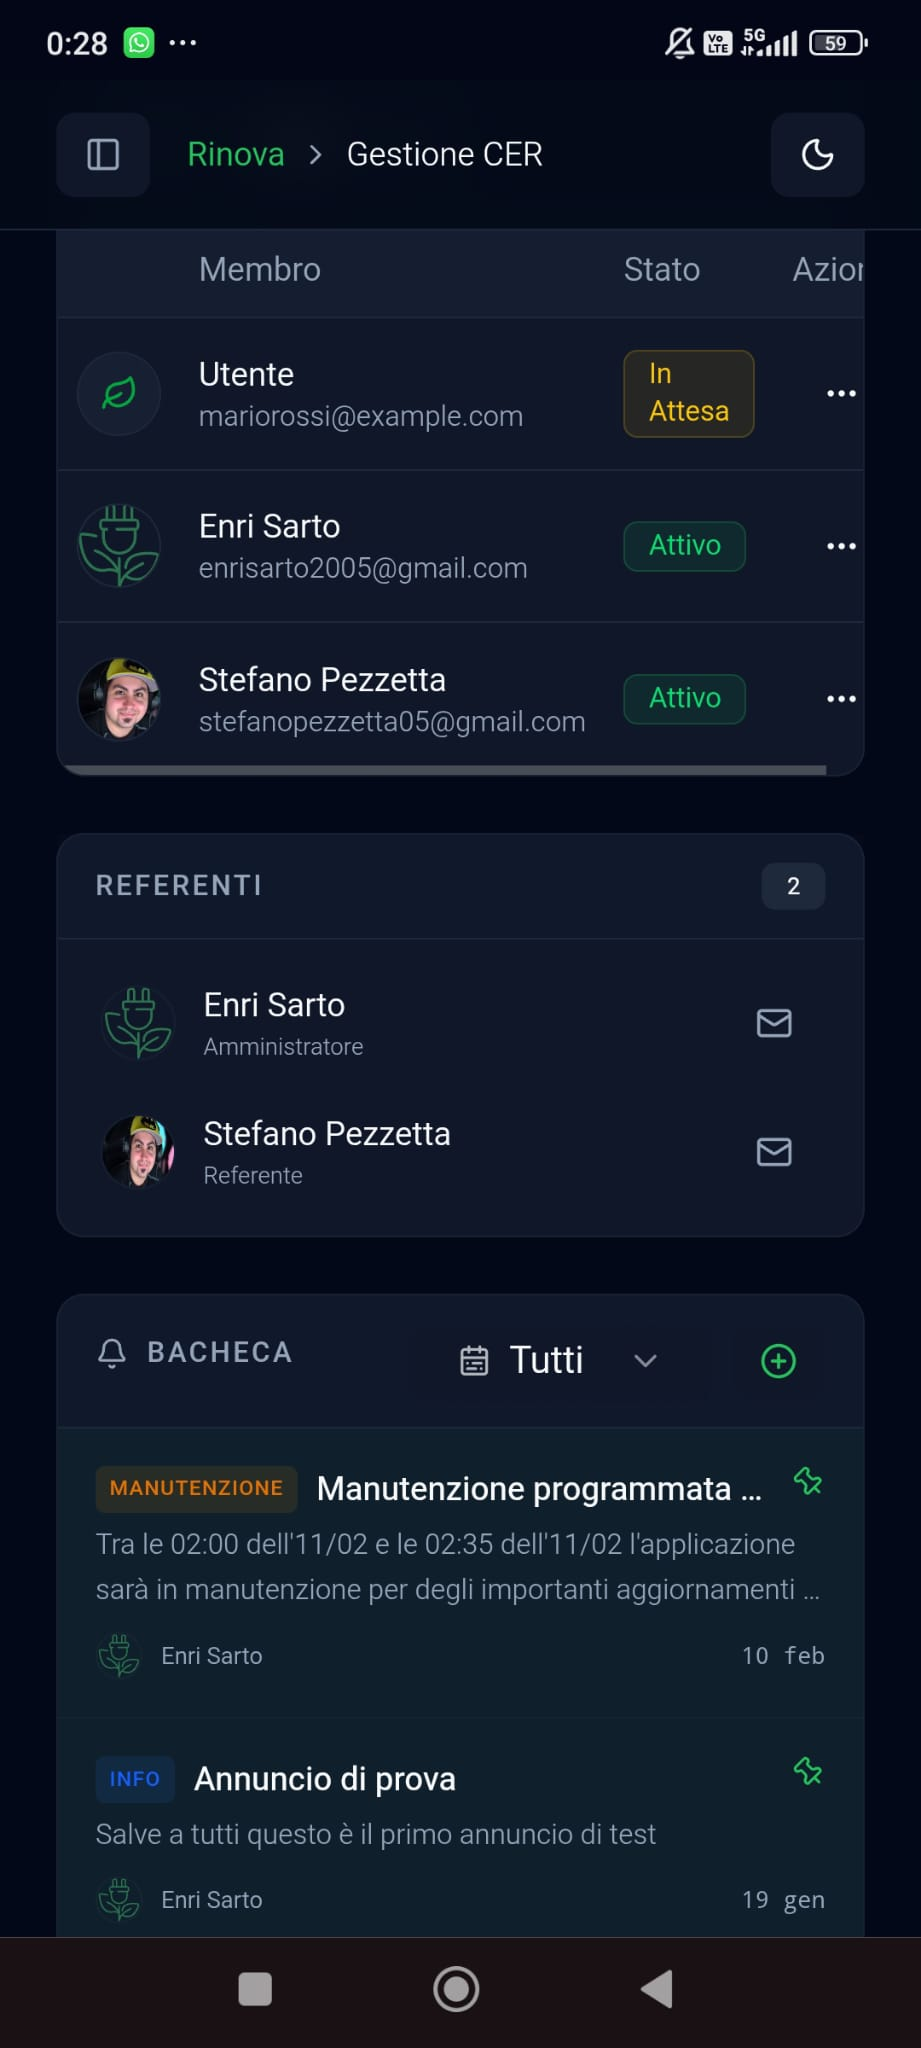
\includegraphics[width=0.35\textwidth]{images/frontend/mobile/cer_mobile_dark.jpeg}
    
    \caption{Gestione CER: Vista Desktop (sopra) e Vista Mobile (sotto). MVP per l'amministrazione della bacheca e dei ruoli della comunità, ottimizzato per entrambi i dispositivi.}
\end{figure}